\documentclass{subfiles}
\begin{document}

\section{Entanglement}
The concept of entanglement is a fundamental feature of quantum mechanical systems, distinguishing interacting quantum systems from classical systems. Conceptually introduced by Einstein, Podolski, and Rosen in their 1935 EPR paper \cite{EPR_1935}, the term \emph{entanglement} was later formalized by Schrödinger in the same year \cite{Schrödinger_1935}. Entanglement measures the correlations between two or more quantum mechanical subsystems. Any system with more than one degree of freedom exhibits such correlations between the "allowed states" in the system, and these correlations make the system non-separable. This means that, even if we have a complete description of the full system, we may not have a complete description of the correlated (entangled) subsystems. For a system of multiple particles, this implies that the state of each particle cannot be described independently of the states of the other particles, even if they are spatially separated by large distances. As Einstein famously expressed, there exists what he referred to as \emph{"spooky action at a distance"}, a phenomenon that classical physics fails to explain or replicate.\\ \\
\subsection{Bell states}
In our system, we will be working in a bipartite system. This means that we have two subsystems, $L$ and $R$ (left and right), which are connected by a coupling Hamiltonian. Our two subsystems are two electrically charged particles, each trapped in a Morse potential well \textcolor{red}{ref til Morse potential bilde av systemet}, which then are coupled through the Coulomb interaction. 
To illustrate the concept of entanglement, we can consider a simple example of two distinguishable particles, $A$ and $B$, in a two-particle system, with two available states in each subsystem (ground state and excited state). The state of the system can be expressed as a product state, where each particle is in a separate state:
\begin{align*}
    \ket{\Psi} = \ket{\psi_A}\otimes\ket{\psi_B}
\end{align*}
where the available states are $\ket{\psi_A} = \ket{0} \text{or} \ket{1}$ and $\ket{\psi_B} = \ket{0} \text{or} \ket{1}$. The system can be in any of the four possible product states: 
\begin{align*}
    \ket{00} = \ket{0}_A\otimes\ket{0}_B, \quad \ket{01} = \ket{0}_A\otimes\ket{1}_B, \\
    \ket{10} = \ket{1}_A\otimes\ket{0}_B, \quad \ket{11} = \ket{1}_A\otimes\ket{1}_B
\end{align*}
However, due to the influence of the coupling Hamiltonian, the system can evolve into an entangled state, in which the state of the particles are mutually dependent. An example of such entangled states are the Bell states, which are maximally entangled states of two qubits. These states are given by
\begin{align*}
    \ket{\Phi^+} &= \frac{1}{\sqrt{2}}(\ket{00} + \ket{11}) \\
    \ket{\Phi^-} &= \frac{1}{\sqrt{2}}(\ket{00} - \ket{11}) \\
    \ket{\Psi^+} &= \frac{1}{\sqrt{2}}(\ket{01} + \ket{10}) \\
    \ket{\Psi^-} &= \frac{1}{\sqrt{2}}(\ket{01} - \ket{10})
\end{align*}
\\ 
In these states, measurements of the state of particle $A$ will immediately give information about the state in which particle $B$ is in, and vice versa. For example, if we prepare our systm in the Bell state $\ket{\Phi^+}$ and measure particle $A$ and find it in the state $\ket{0}$, we can immediately conclude that particle $B$ is also in the state $\ket{0}$. This is a fact, regardless of the physical separation of the two particles and was the basis for the EPR paradox \cite{EPR_1935}. This phenomenon, entanglement, is a direct consequence of the non-locality of quantum mechanics, and is a key resource for many quantum technologies, such as quantum computing, quantum cryptography, and quantum teleportation.\textcolor{red}{find sources}\\ 

\subsection{Quantifying, and measuring entanglement}
While entanglement is conceptually well understood, quantifying it in physical systems - especially continuous and/or spatially extended systems like ours - requires precise mathematical tools. In our system of two charged particles confined in a double Morse well system (\textcolor{red}{Ref til Morse}), we aim to characterize the degree of entanglement between subsystems $L$ and $R$ that emerges due to the Coulomb coupling. To accomplish this, we shall turn to established entanglement measures such as the \emph{von Neumann entropy}, which will allow us to quantify the extent to which subsystms $L$ and $R$ are entangled. To do so, we will also introduce the concept of the reduced density matrix and explore it's physical intepretation in the context of our bipartite system.
\\ \\
In classical physics, we always assume the system to exists in well-defined, definite states, with any uncertainty arising solely from a \emph{lack of information or knowledge}. For example, a certain object will have a specific location in phase space, regardless of our knowledge of what this location is. This is what we call \emph{pure states}. States that give a complete and unambigous description of the system. In quantum mechanics the situation is more nuanced. While there are systems that can be described by such pure states (and represented by a single state vector), many systems require a more general description, particularly large entangled systems of subsystems. In such cases, while the entire system as a whole is in a well-defined quantum state, the smaller subsystems may not have definite states of their own. Instead they can exists in a \emph{mixed state}, which represents a statistical mixture - an ensamble - of different possible (pure) quantum states.
To summarize, a mixed state is a probabilistic combination of pure states, where the system is in one of the pure states with a certain probability. This is a direct consequence of the entanglement between the subsystems, as the correlations between them lead to uncertainty in the description of each subsystem. As opposed to the classical uncertainty, which arises from a lack of information, the uncertainty in quantum mechanics is a fundamental property of the system itself. This means that even if we have complete knowledge of the entire system, and it exists in a pure state, we may not be able to assign definite states to the subsystems meaning they are in mixed states. 
\\ \\ 
Thus describing these mixtures require a more general formalism, and to do so we introduce the \emph{density matrix formalism}. First introduced by John von Neumann in 1927\cite{neumann1927}, the density matrix formalism allows for expressing quantum states by both pure and mixed states and it's an essential tool for understanding and quantifying entanglement, since it encapsulates information about how a subsystem becomes "uncertain" due to its correlations with the rest of the system. As a representation of the \emph{density operator}, which the two terms in practice are used interchangeably, the density matrix (operator) is given as
\begin{equation}
    \rho = \sum_i w_i\ket{\psi_i}\bra{\psi_i}\label{eq:density_matrix}
\end{equation}
where the probability weight $w_i$ is the probability of finding the system in the pure state $\ket{\psi_i}$. The density matrix is a positive semi-definite operator, and it has the following properties:
\begin{itemize}
    \item $\text{Tr}(\rho) = 1$, meaning the trace of the density matrix is equal to 1, given that $\rho$ is a pure state. $\text{Tr}(\rho) < 1$ for mixed states.
    \item $\rho^\dagger = \rho$, meaning the density matrix is Hermitian.
    \item $\rho \geq 0$, meaning the density matrix is positive semi-definite.
\end{itemize}
Returning to our simple system of two distinguishable particles, we can express the density matrix of the system as
\begin{align*}
    \rho_{AB} = \begin{pmatrix}
        \rho_{00, 00} & \rho_{00, 01} & \rho_{00, 10} & \rho_{00, 11} \\
        \rho_{01, 00} & \rho_{01, 01} & \rho_{01, 10} & \rho_{01, 11} \\
        \rho_{10, 00} & \rho_{10, 01} & \rho_{10, 10} & \rho_{10, 11} \\
        \rho_{11, 00} & \rho_{11, 01} & \rho_{11, 10} & \rho_{11, 11}
    \end{pmatrix}
\end{align*}
where the diagonal elements of the density matrix are the probability populations of the system being in the corresponding states $\ket{00}, \ket{01}, \ket{10}, \ket{11}$, while the off-diagonal elements are the coherences between said states - signatures of superposition states. Such superposition states differ from mixed states, as they are not statistical mixtures of pure states, but rather linear combinations of pure states. But how do we measure the entanglement in our system? To do so, we've mentioned the von Neumann entropy, which is a measure of the amount of information that is missing from the system. The von Neumann entropy is defined as
\begin{equation}
    S(\rho) = -\text{Tr}(\rho \ln \rho)
\end{equation}
where $\rho$ is the density matrix of the system. But how do we relate this to entanglement when working with multiple entangled subsystems? We then need to find the \emph{reduced density matrix}, which is a partial trace of the full density matrix over the other subsystem. Effectively, this means we are tracing out (or removing) the degrees of freedom in the other subsystems, which do not directly contribute to the entanglement. The reduced density matrix for subsystem $A$ is given as
\begin{equation}
    \rho_A = \text{Tr}_B(\rho_{AB}) = \sum_{i}\bra{i_B}\rho_{AB}\ket{i_B}
\end{equation}
where $\ket{i_B}$ are the basis states of subsystem $B$. The reduced density matrix for subsystem $B$ is given in a similar manner. The von Neumann entropy of the reduced density matrix is then given as
\begin{equation}
    S(\rho_A) = -\text{Tr}(\rho_A \ln \rho_A)
\end{equation}
and it can easily be shown that $S(\rho_A) = S(\rho_B)$, meaning the entanglement is symmetric between the two subsystems, which is to be expected. 


\\\\ 
Another useful aspect of the density matrix formalism is that it naturally ties together with measurements in quantum mechanics. Let us consider a quantum system expressed by a density matrix $\rho$ as in \eqref{eq:density_matrix}, and we want to measure an observable $O$ in the system. The expectation value of the observable is given as
\begin{align*}
    \braket{O} = \sum_i w_i\bra{\psi_i}O\ket{\psi_i} = \sum_i w_i\text{Tr}\big(\ket{\psi_i}\bra{\psi_i}O\big) = \text{Tr}\big(\sum_i w_i \ket{\psi_i}\bra{\psi_i}O\big) = \text{Tr}(\rho O)
\end{align*}
and we see how powerful this notation is, we can quickly calculate expectation values of operators (observables) by a simple trace operation. 

\subsection{Avoided crossings}\label{sec:avoided_crossings}
In our coupled, double well system \eqref{eq:double_well_morse_potential}, the emergence of entanglement is a direct consequence of the Coulomb coupling between the two subsystems. This coupling will give rise to a phenomenon known as \emph{avoided crossings}\cite{nazir2005anticrossings}, regions in the parameter space where the energy levels of the two subsystems come close to each other, but do not cross due to the coupling of the two subsystems. This coupling makes it so that the energy levels that may be degenerate in the uncoupled system, are no longer degenerate in the coupled system and they are no longer independent, and the system is no longer separable or expressable as a product state. This means our two subsystems will be entangled, and the energy levels will be shifted due to the coupling and this we can use to manipulate the system. \\ \\
To illustrate this, we can consider a simple example of a two level system, with two energy levels $E_1$ and $E_2$, which are degenerate in the uncoupled system, i.e $E_1 = E_2$. Introducing a coupling term $V$, the effective Hamiltonian of the system can be expressed as
\begin{align*}
    H = \begin{pmatrix}
        E_1 & V \\
        V & E_2
    \end{pmatrix}
\end{align*}
where $V$ is the coupling strength between the two levels. The eigenvalues of this Hamiltonian are given as
\begin{align*}
    E_\pm = \frac{E_1 + E_2}{2} \pm \sqrt{\frac{(E_1 - E_2)^2}{4} + V^2}
\end{align*}
and we can see that the energy levels are shifted due to the coupling, and they will never cross for $V\neq0$. \\ \\

Consider now a dynamical system, where there is some explicit time-dependence in the Hamiltonian, with a constant coupling strength $V$.
\begin{align}
    H(t) = \begin{pmatrix}
        E(t) & V \\
        V & -E(t)
    \end{pmatrix} = \begin{pmatrix}
        vt & V \\
        V & -vt
    \end{pmatrix} \label{eq:landau_zener}
\end{align}
where $E(t)$ is the time-dependent energy level of the system, with $v$ the sweeping parameter, that sweep the energy levels towards each other (they are equal at $t=0$). 

Simulating for a time starting from $t<0$, where the energy levels are degenerate we will highlight the avoided crossing at $t=0$, and we get what is called a \emph{Landau-Zener transition} \cite{landau1932theorie, zener1932non}. 
\begin{figure}[h!]
    \centering
    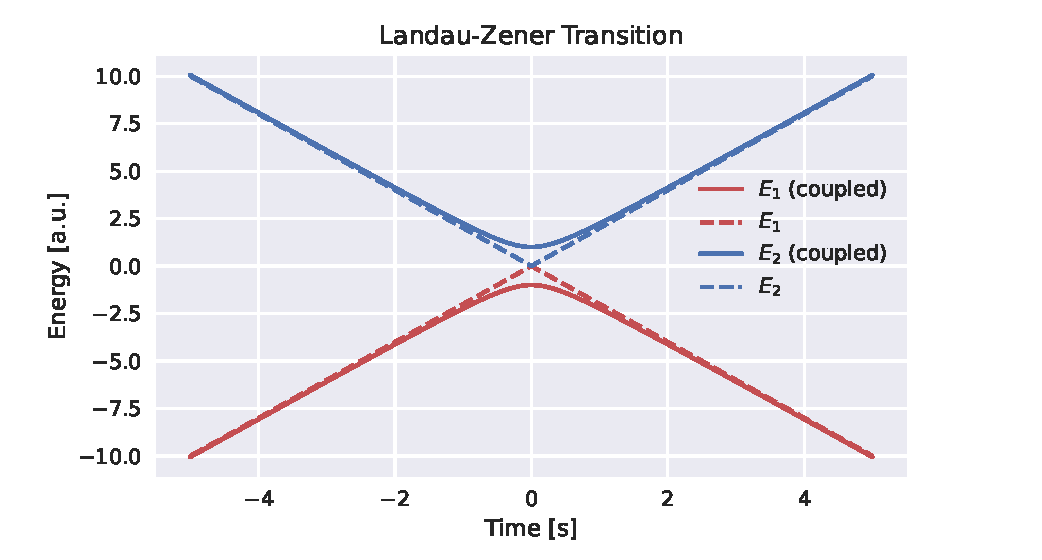
\includegraphics[width=0.8\textwidth]{figs/avoided_crossing.pdf}
    \caption{The avoided crossings in a two-level system as a function time $t$. The energy levels are shifted due to the coupling, and the energy levels do not cross, but rather "avoid" each other.}
    \label{fig:avoided_crossings}
\end{figure}
As we can see, the Coulomb coupling between the two subsystems results in the energy levels 'avoiding' eachother, while the non-interacting system would have crossed at $t=0$ (as indicated by the dotted lines). But what happens with the wavefunctions prepared in th system? Initializing the system in the ground state $\psi_0 = \ket{0}$, we shall see that what happens at the avoided crossing depends heavily on both coupling strength $V$ and sweeping paramter $k$, through the Landau-Zener formula \cite{landau1932theorie, zener1932non}:
\begin{align}
    P_{0\rightarrow1} = e^{-\frac{2\pi V^2}{\hbar k}}\label{eq:landau_zener_trans_prob}
\end{align}
which governs the probability of the system to transitions between the two energy levels. As visualized in the following plot \eqref{fig:landau_zener}, we can see how the sweeping parameter $k$ governs how the avoided crossing affect the prepared wavefunction, in one case we achive some minor level of mixing between the two basis states, while in the other case we achieve a full transition between the two states.
\begin{figure}[h!]
    \centering
    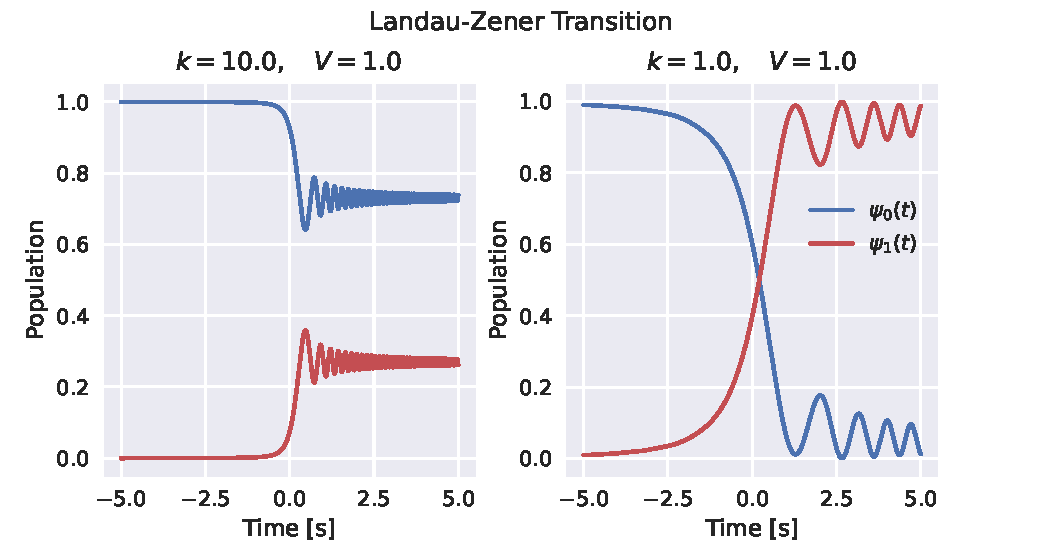
\includegraphics[width=0.8\textwidth]{figs/landau_zener.pdf}
    \caption{The Landau-Zener transition probability as a function of the coupling strength $V$ and the sweeping parameter $k$. The probability of the system to transition between the two energy levels is given by the Landau-Zener formula.}
    \label{fig:landau_zener}
\end{figure} 

\\ \\

\begin{itemize}
    \item What is entanglement
    \item Why is it important
    \item How do we measure it
    \item How do we create it
    \item How do we use it - avoided crossings, ref \cite{nazir2005anticrossings}
\end{itemize}



\end{document}